%%%%%%%%%%%%%%%%%%%%%%%%%%%%%%%%%%%%%%%%%%%%%%%%%%%%%%%%%%%%%%%%%%%%%%%%%%%%%%%%%%
\begin{frame}[fragile]\frametitle{}
\begin{center}
{\Large Introduction}
\end{center}
\end{frame}

%%%%%%%%%%%%%%%%%%%%%%%%%%%%%%%%%%%%%%%%%%%%%%%%%%%%%%%%%%%
\begin{frame}[fragile]\frametitle{What Are Mental Models?}
      \begin{itemize}
        \item Mental Models help us understand and interpret the world.
        \item They shape how we think, what we notice, and what we ignore.
        \item Mental Models simplify complexity and highlight relevance.
        \item They guide reasoning, decision-making, and perception.
        \item Every thought process relies on some form of Mental Model.
      \end{itemize}
\end{frame}

%%%%%%%%%%%%%%%%%%%%%%%%%%%%%%%%%%%%%%%%%%%%%%%%%%%%%%%%%%%
\begin{frame}[fragile]\frametitle{Mental Models: From Data to Knowledge}
      \begin{itemize}
        \item Information = raw data.
        \item Thinking = organizing information into structure.
        \item Knowledge = structured information with meaning.
        \item Mental Models are structured knowledge frameworks.
        \item They convert data into insight by imposing structure and meaning.
      \end{itemize}
	  
	\begin{center}
	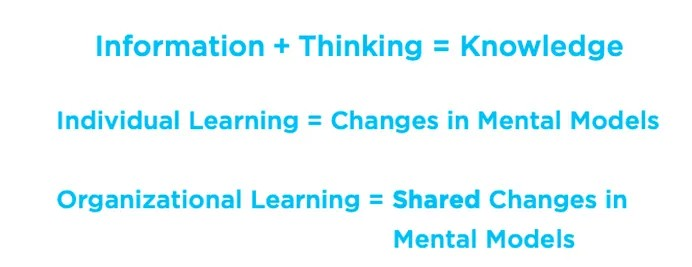
\includegraphics[width=0.8\linewidth,keepaspectratio]{mm3}
	\end{center}
	
{\tiny (Ref: The Art Of Thinking Clearly - Swabhav Tech Labs)}  	  
\end{frame}

%%%%%%%%%%%%%%%%%%%%%%%%%%%%%%%%%%%%%%%%%%%%%%%%%%%%%%%%%%%
\begin{frame}[fragile]\frametitle{Example: Paradigm Shift}
      \begin{itemize}
        \item ``Paradigm Shift'' is a Mental Model for deep systemic change.
        \item It describes a total shift in how a subject is understood.
        \item Encourages openness to change and challenging assumptions.
        \item Used in science, business, and personal development.
        \item Helps recognize when old models no longer explain new realities.
      \end{itemize}
\end{frame}

%%%%%%%%%%%%%%%%%%%%%%%%%%%%%%%%%%%%%%%%%%%%%%%%%%%%%%%%%%%
\begin{frame}[fragile]\frametitle{What Is Mental Model Thinking?}
      \begin{itemize}
        \item Applying multiple models to interpret and solve problems.
        \item Helps identify patterns and structure information efficiently.
        \item Enhances insight, clarity, and decision-making.
        \item Encourages flexible and adaptive thinking.
        \item Widely used in strategy, systems thinking, and learning.
      \end{itemize}
\end{frame}

%%%%%%%%%%%%%%%%%%%%%%%%%%%%%%%%%%%%%%%%%%%%%%%%%%%%%%%%%%%
\begin{frame}[fragile]\frametitle{Mental Models in Learning}
      \begin{itemize}
        \item Learning forms internal frameworks called Mental Models.
        \item These models help organize, relate, and apply new knowledge.
        \item Prior experience shapes how new models are formed.
        \item Models evolve through active engagement and reflection.
        \item Teachers can help learners by fostering model-building skills.
      \end{itemize}
\end{frame}

%%%%%%%%%%%%%%%%%%%%%%%%%%%%%%%%%%%%%%%%%%%%%%%%%%%%%%%%%%%
\begin{frame}[fragile]\frametitle{Building Better Mental Models}
      \begin{itemize}
        \item Seek diverse models to gain richer perspectives.
        \item Continuously test and refine your mental frameworks.
        \item Discard models that no longer serve or predict well.
        \item Use models as tools, not truths.
        \item Read Farnam Street's ``The Great Mental Models'' is a great start.
      \end{itemize}
\end{frame}



%%%%%%%%%%%%%%%%%%%%%%%%%%%%%%%%%%%%%%%%%%%%%%%%%%%%%%%%%%%
\begin{frame}[fragile]\frametitle{Introduction to Mental Models}
  \begin{itemize}
    \item Mental models are frameworks to simplify complex decision-making.
    \item Popularized by Charlie Munger and Shane Parrish.
    \item Originates from cognitive psychology and systems theory.
    \item Helps in investing (e.g., Munger's latticework), policymaking, and life choices.
    \item E.g., Ratan Tata applying mental models in Tata Nano's design.
    \item Be aware of over-relying on one model; use a toolbox approach.
  \end{itemize}
\end{frame}

%%%%%%%%%%%%%%%%%%%%%%%%%%%%%%%%%%%%%%%%%%%%%%%%%%%%%%%%%%%
\begin{frame}[fragile]\frametitle{Why Do We Have Mental Models?}
      \begin{itemize}
        \item Brains evolved to predict environmental changes and increase survival odds.
        \item Mental Models are tools the brain uses to make accurate predictions.
        \item Decision-making is based on predictions, consciously or subconsciously.
        \item Mental Models help assign meaning to experiences and emotions.
        \item We use them in both logical decisions and emotional interpretations.
        \item Even basic reactions (e.g. Fight or Flight) are driven by primal models.
        \item Mental Models fill gaps in uncertainty to help us make sense of the world.
      \end{itemize}
\end{frame}

%%%%%%%%%%%%%%%%%%%%%%%%%%%%%%%%%%%%%%%%%%%%%%%%%%%%%%%%%%%
\begin{frame}[fragile]\frametitle{Mental Models as Predictive Tools}
      \begin{itemize}
        \item All decisions are bets on Mental Model-based predictions.
        \item Models like 80/20 or Second Order Thinking predict system outcomes.
        \item Mental Models help evaluate probabilities in uncertain environments.
        \item They convert external stimuli into internal meaning and action.
        \item Interpretation of social cues often uses layered Mental Models.
        \item Miscalibrated models can lead to incorrect assumptions and behavior.
        \item Models operate both reactively (instinct) and reflectively (consciously).
        \item They underpin both logical reasoning and emotional reactions.
      \end{itemize}
\end{frame}

%%%%%%%%%%%%%%%%%%%%%%%%%%%%%%%%%%%%%%%%%%%%%%%%%%%%%%%%%%%
\begin{frame}[fragile]\frametitle{Five Cognitive Dimensions of Mental Models}
      \begin{itemize}
        \item Instinct – hard-coded evolutionary models like Fight or Flight.
        \item Faith – belief-based models rooted in tradition, religion, and myth.
        \item Preference – ego-driven models shaped by desire, ideology, and culture.
        \item Logic – models based on reasoned inductive arguments and observation.
        \item Evidence – models validated through experience or experimentation.
      \end{itemize}
\end{frame}

%%%%%%%%%%%%%%%%%%%%%%%%%%%%%%%%%%%%%%%%%%%%%%%%%%%%%%%%%%%
\begin{frame}[fragile]\frametitle{Cognitive Dimensions}
	
	\begin{center}
	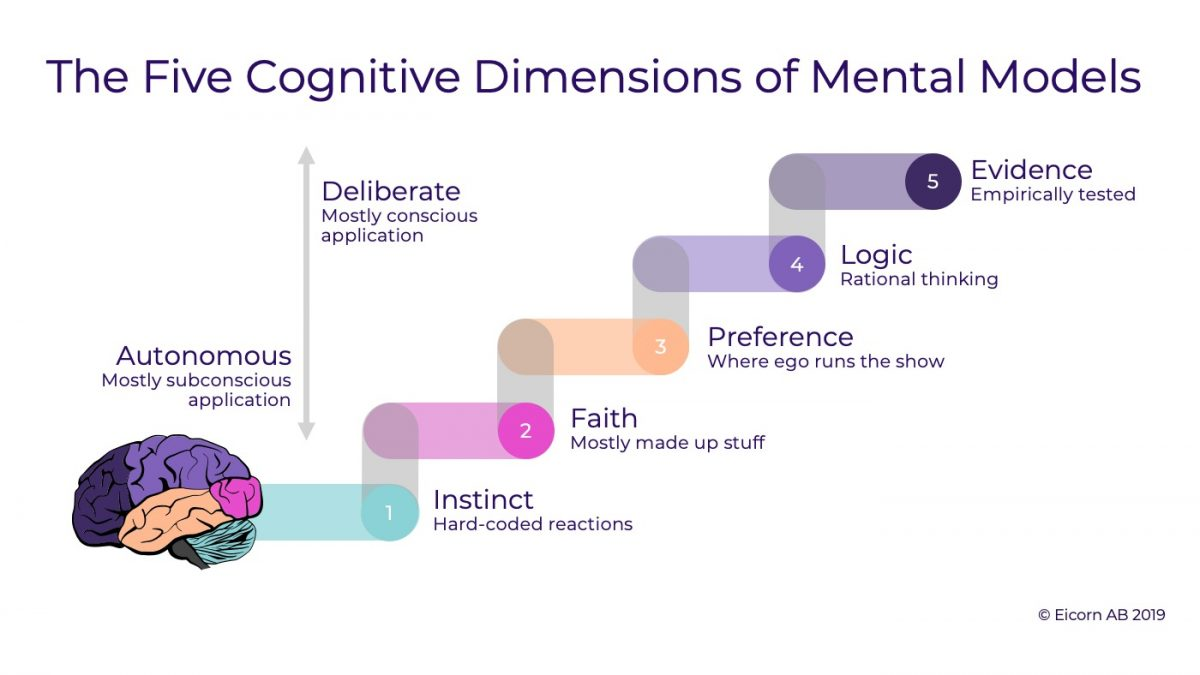
\includegraphics[width=\linewidth,keepaspectratio]{mm1}
	\end{center}
	
{\tiny (Ref: The Architecture of Mental Models - Eicorn)}

\end{frame}


%%%%%%%%%%%%%%%%%%%%%%%%%%%%%%%%%%%%%%%%%%%%%%%%%%%%%%%%%%%
\begin{frame}[fragile]\frametitle{Instinct-Based Mental Models}
      \begin{itemize}
        \item Instincts are primal and evolutionarily hardwired.
        \item Fight or Flight is a classic example of this dimension.
        \item Responses are automatic and cannot be reprogrammed directly.
        \item We can only train our reactions to instinctive triggers.
        \item These models are ancient, deep-seated, and difficult to override.
      \end{itemize}
\end{frame}

%%%%%%%%%%%%%%%%%%%%%%%%%%%%%%%%%%%%%%%%%%%%%%%%%%%%%%%%%%%
\begin{frame}[fragile]\frametitle{Faith-Based Mental Models}
      \begin{itemize}
        \item Built on beliefs, not necessarily evidence or logic.
        \item Often found in religious or cultural origin stories.
        \item Meaningful for many, but poor predictors of reality.
        \item Highly changeable,we can choose to revise or discard them.
        \item Some thinkers maintain faith models for meaning, not logic.
      \end{itemize}
\end{frame}

%%%%%%%%%%%%%%%%%%%%%%%%%%%%%%%%%%%%%%%%%%%%%%%%%%%%%%%%%%%
\begin{frame}[fragile]\frametitle{Preference-Based Mental Models}
      \begin{itemize}
        \item Shaped by ego, ideology, wishful thinking, and group norms.
        \item Often distort reality to match desires or identity.
        \item Tribalism and stubbornness emerge from these models.
        \item Social compliance reinforces many preference-based models.
        \item Often inherited from past belief systems or cultures.
      \end{itemize}
\end{frame}

%%%%%%%%%%%%%%%%%%%%%%%%%%%%%%%%%%%%%%%%%%%%%%%%%%%%%%%%%%%
\begin{frame}[fragile]\frametitle{Logic-Based Mental Models}
      \begin{itemize}
        \item Built from reasoning and inductive observation.
        \item Rooted in philosophy and early scientific thought (e.g. Logos).
        \item Theories and hypotheses form the basis of these models.
        \item Vulnerable to inductive errors, but very useful when crafted well.
        \item Common in science, business strategy, and critical thinking.
      \end{itemize}
\end{frame}

%%%%%%%%%%%%%%%%%%%%%%%%%%%%%%%%%%%%%%%%%%%%%%%%%%%%%%%%%%%
\begin{frame}[fragile]\frametitle{Evidence-Based Mental Models}
      \begin{itemize}
        \item Built from tested logic and real-world outcomes.
        \item Most accurate and useful for understanding reality.
        \item Examples: multitasking is inefficient; 80/20 works in specific domains.
        \item Can be misapplied if overgeneralized beyond the evidence.
        \item Critical to distinguish between tested truth and inductive guesswork.
      \end{itemize}
\end{frame}




%%%%%%%%%%%%%%%%%%%%%%%%%%%%%%%%%%%%%%%%%%%%%%%%%%%%%%%%%%%%%%%%%%%%%%%%%%%%%%%%%%
\begin{frame}[fragile]\frametitle{}
\begin{center}
{\Large Mental Models}
\end{center}
\end{frame}

%%%%%%%%%%%%%%%%%%%%%%%%%%%%%%%%%%%%%%%%%%%%%%%%%%%%%%%%%%%
\begin{frame}[fragile]\frametitle{First Principles Thinking}
  \begin{itemize}
    \item Break problems down to their fundamental truths.
    \item Originates from Aristotle and physics.
    \item Used in startups, e.g., Ola dissecting cab logistics vs. copying taxi systems.
    \item In cooking, understanding base ingredients vs. recipes.
    \item E.g., ISRO's cost-effective Mars mission using fundamental physics and constraints.
    \item Beware of ignoring proven heuristics and reinventing unnecessarily.
  \end{itemize}
  
	\begin{center}
	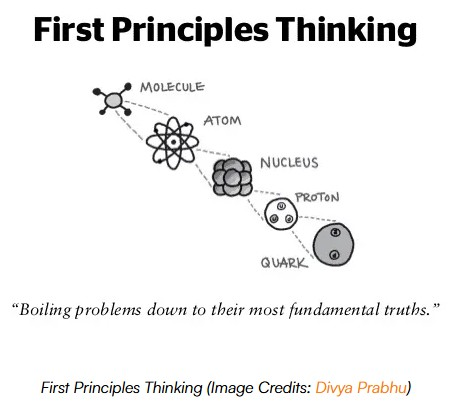
\includegraphics[width=0.5\linewidth,keepaspectratio]{mm6}
	\end{center}
	
{\tiny (Ref: The Art Of Thinking Clearly - Swabhav Tech Labs)}      
\end{frame}

%%%%%%%%%%%%%%%%%%%%%%%%%%%%%%%%%%%%%%%%%%%%%%%%%%%%%%%%%%%
\begin{frame}[fragile]\frametitle{Inversion}
  \begin{itemize}
    \item Thinking in reverse , ``what would cause failure?''
    \item Inspired by Carl Jacobi's ``invert, always invert.''
    \item In finance: prevent loss before seeking gain.
    \item In daily life: avoiding bad health rather than only pursuing good.
    \item E.g., B-schools teaching case studies of failed Indian startups.
    \item Avoid over-focusing on negatives; it's a tool, not a worldview.
  \end{itemize}
  
	\begin{center}
	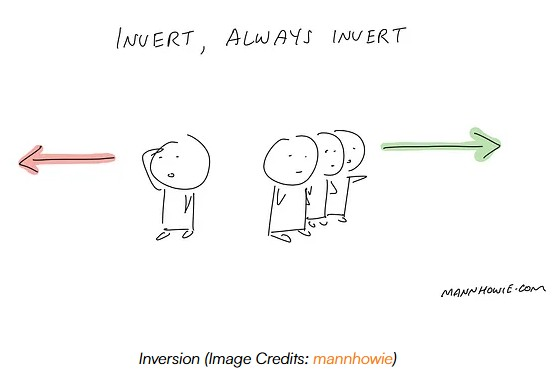
\includegraphics[width=\linewidth,keepaspectratio]{mm10}
	\end{center}
	
{\tiny (Ref: The Art Of Thinking Clearly - Swabhav Tech Labs)}    
\end{frame}

%%%%%%%%%%%%%%%%%%%%%%%%%%%%%%%%%%%%%%%%%%%%%%%%%%%%%%%%%%%
\begin{frame}[fragile]\frametitle{Opportunity Cost}
  \begin{itemize}
    \item Cost of the next best alternative foregone.
    \item Core principle in economics since classical era.
    \item Choosing civil services over entrepreneurship , missed upside.
    \item In Indian agriculture: water for paddy vs. cash crops.
    \item E.g., investor choosing fixed deposit vs. equity.
    \item Don't ignore hidden or non-financial costs; measure holistically.
  \end{itemize}
\end{frame}

%%%%%%%%%%%%%%%%%%%%%%%%%%%%%%%%%%%%%%%%%%%%%%%%%%%%%%%%%%%
\begin{frame}[fragile]\frametitle{Second-Order Thinking}
  \begin{itemize}
    \item Anticipating consequences of consequences.
    \item Key to systems thinking; used by top strategists.
    \item In politics: free electricity → higher consumption → grid stress.
    \item In business: discounts → loss leaders → brand erosion.
    \item E.g., UPI adoption → cashless economy → surveillance concerns.
    \item Avoid paralysis by analysis; balance depth with action.
  \end{itemize}
  
	\begin{center}
	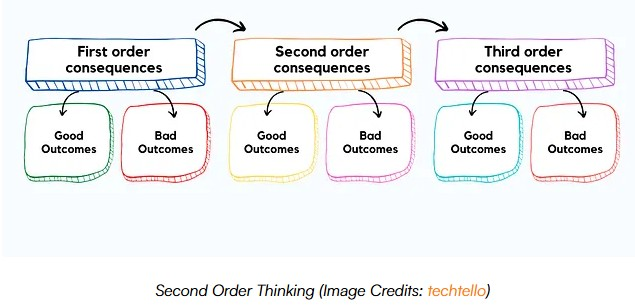
\includegraphics[width=\linewidth,keepaspectratio]{mm8}
	\end{center}
	
{\tiny (Ref: The Art Of Thinking Clearly - Swabhav Tech Labs)}      
\end{frame}

%%%%%%%%%%%%%%%%%%%%%%%%%%%%%%%%%%%%%%%%%%%%%%%%%%%%%%%%%%%
\begin{frame}[fragile]\frametitle{The Map is Not the Territory}
  \begin{itemize}
    \item Models are simplifications , not reality itself.
    \item Coined by Alfred Korzybski, popular in systems science.
    \item GDP $\neq$ actual prosperity; rankings $\neq$ real competence.
    \item E.g., exam scores $\neq$ intelligence; IRCTC waitlist $\neq$ travel reality.
    \item E.g., BPL card $\neq$ real poverty in rural India.
    \item Don't confuse labels or proxies with full understanding.
  \end{itemize}
  
	\begin{center}
	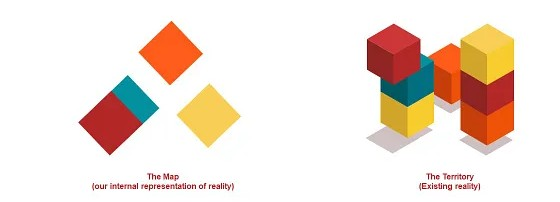
\includegraphics[width=0.5\linewidth,keepaspectratio]{mm4}
	\end{center}
	
{\tiny (Ref: The Art Of Thinking Clearly - Swabhav Tech Labs)}  	 
\end{frame}

%%%%%%%%%%%%%%%%%%%%%%%%%%%%%%%%%%%%%%%%%%%%%%%%%%%%%%%%%%%
\begin{frame}[fragile]\frametitle{Circle of Competence}
  \begin{itemize}
    \item Know what you know , and what you don't.
    \item Warren Buffett's key idea; deeply tied to humility.
    \item Investors stick to known sectors , pharma vs. tech.
    \item E.g., Indian cricket team sticking to seamers on green pitches.
    \item E.g., Byju's scaling fast in edtech, failed in physical schools.
    \item Don't make your circle too small , be open to learning.
  \end{itemize}
  
	\begin{center}
	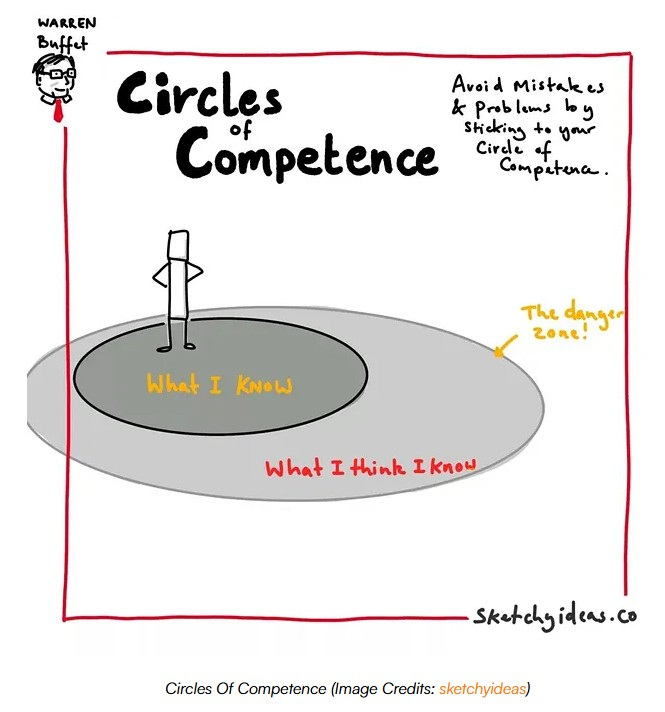
\includegraphics[width=0.5\linewidth,keepaspectratio]{mm5}
	\end{center}
	
{\tiny (Ref: The Art Of Thinking Clearly - Swabhav Tech Labs)}    
\end{frame}

%%%%%%%%%%%%%%%%%%%%%%%%%%%%%%%%%%%%%%%%%%%%%%%%%%%%%%%%%%%
\begin{frame}[fragile]\frametitle{Ockham's Razor}
  \begin{itemize}
    \item Simplest explanation is often correct.
    \item Named after William of Ockham, 14th century.
    \item Used in diagnosis, journalism, and science.
    \item E.g., missing train due to traffic vs. conspiracy by cabbie.
    \item E.g., Aadhaar leaks more likely due to mismanagement than espionage.
    \item Beware of oversimplification; simple $\neq$ accurate.
  \end{itemize}
  
	\begin{center}
	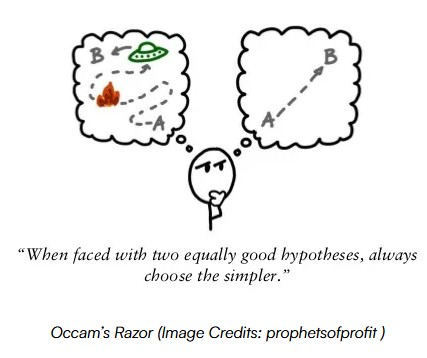
\includegraphics[width=0.6\linewidth,keepaspectratio]{mm11}
	\end{center}
	
{\tiny (Ref: The Art Of Thinking Clearly - Swabhav Tech Labs)}     
\end{frame}

%%%%%%%%%%%%%%%%%%%%%%%%%%%%%%%%%%%%%%%%%%%%%%%%%%%%%%%%%%%
\begin{frame}[fragile]\frametitle{The Lindy Effect}
  \begin{itemize}
    \item The longer something survives, the longer it's likely to.
    \item Popularized by Nassim Taleb; derived from theater.
    \item Sanskrit, Ayurveda , resilient knowledge in Indian context.
    \item Brands like Amul, Tata indicate trust through time.
    \item E.g., epics like Mahabharata enduring cultural relevance.
    \item New $\neq$ better; but old $\neq$ always useful , evaluate critically.
  \end{itemize}
\end{frame}

%%%%%%%%%%%%%%%%%%%%%%%%%%%%%%%%%%%%%%%%%%%%%%%%%%%%%%%%%%%
\begin{frame}[fragile]\frametitle{Sunk Cost Fallacy}
  \begin{itemize}
    \item Continuing due to past investment, not future value.
    \item Studied in behavioral economics.
    \item Government projects continued despite low returns.
    \item E.g., B-school student finishing MBA despite hating it.
    \item E.g., personal relationships carried forward ``because of time invested.''
    \item Don't throw good money (or time) after bad.
  \end{itemize}
\end{frame}

%%%%%%%%%%%%%%%%%%%%%%%%%%%%%%%%%%%%%%%%%%%%%%%%%%%%%%%%%%%
\begin{frame}[fragile]\frametitle{The Pareto Principle (80/20 Rule)}
  \begin{itemize}
    \item 80% of results come from 20% of efforts.
    \item Discovered by Vilfredo Pareto in economics.
    \item E.g., 20% of customers bring 80% revenue , common in Indian retail.
    \item In exams, 20% topics cover 80% questions.
    \item E.g., Indian IT firms rely heavily on top 20% of clients.
    \item Avoid ignoring the remaining 80% entirely , edge cases matter.
  \end{itemize}
\end{frame}

%%%%%%%%%%%%%%%%%%%%%%%%%%%%%%%%%%%%%%%%%%%%%%%%%%%%%%%%%%%
\begin{frame}[fragile]\frametitle{Cognitive Biases}
  \begin{itemize}
    \item Systematic deviations from rational thinking.
    \item Studied extensively by Kahneman and Tversky.
    \item Media bias, confirmation bias, anchoring , common in investing and politics.
    \item E.g., brand loyalty despite better alternatives.
    \item Indian voters influenced by recency bias during elections.
    \item Learn biases to spot them, not to feel superior.
  \end{itemize}
\end{frame}

%%%%%%%%%%%%%%%%%%%%%%%%%%%%%%%%%%%%%%%%%%%%%%%%%%%%%%%%%%%
\begin{frame}[fragile]\frametitle{Probabilistic Thinking}
  \begin{itemize}
    \item Thinking in terms of likelihoods, not certainties.
    \item Core to Bayesian reasoning and decision theory.
    \item E.g., cricket match predictions, monsoon forecasts.
    \item Stock investors use expected value calculations.
    \item E.g., Indian RTOs plan road design using accident probabilities.
    \item Avoid overconfidence; even 90% odds fail 1 in 10 times.
  \end{itemize}
  
	\begin{center}
	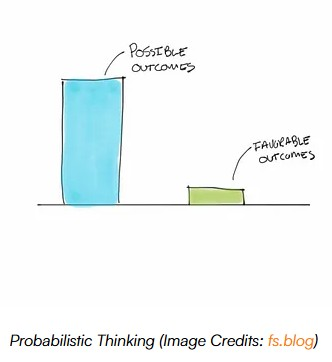
\includegraphics[width=0.5\linewidth,keepaspectratio]{mm9}
	\end{center}
	
{\tiny (Ref: The Art Of Thinking Clearly - Swabhav Tech Labs)}      
\end{frame}

%%%%%%%%%%%%%%%%%%%%%%%%%%%%%%%%%%%%%%%%%%%%%%%%%%%%%%%%%%%
\begin{frame}[fragile]\frametitle{The Dunning-Kruger Effect}
  \begin{itemize}
    \item Incompetent people overestimate their competence.
    \item Coined by psychologists Dunning and Kruger.
    \item E.g., novice trader in India believing they're stock experts post one gain.
    \item Political debates full of loud but uninformed opinions.
    \item E.g., early success of startups can lead to overexpansion.
    \item Competence includes knowing limits; humility is key.
  \end{itemize}
\end{frame}

%%%%%%%%%%%%%%%%%%%%%%%%%%%%%%%%%%%%%%%%%%%%%%%%%%%%%%%%%%%
\begin{frame}[fragile]\frametitle{Hanlon's Razor}
  \begin{itemize}
    \item Never attribute to malice what can be explained by stupidity.
    \item Popular in management and conflict resolution.
    \item E.g., government inefficiency $\neq$ conspiracy.
    \item Indian Railways delays often due to process, not sabotage.
    \item In family arguments, ignorance may explain behavior better than bad intent.
    \item Beware of excusing true malice , discern with care.
  \end{itemize}
  
	\begin{center}
	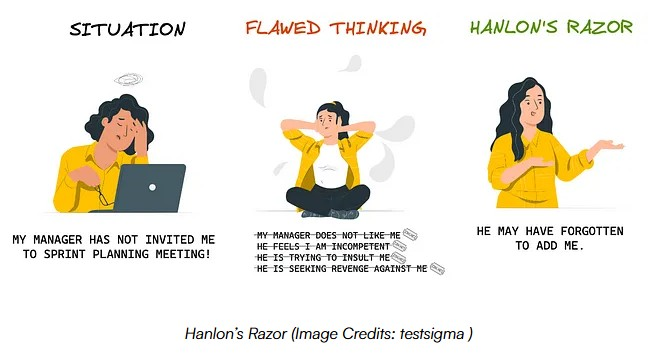
\includegraphics[width=0.8\linewidth,keepaspectratio]{mm12}
	\end{center}
	
{\tiny (Ref: The Art Of Thinking Clearly - Swabhav Tech Labs)}    
\end{frame}

%%%%%%%%%%%%%%%%%%%%%%%%%%%%%%%%%%%%%%%%%%%%%%%%%%%%%%%%%%%
\begin{frame}[fragile]\frametitle{Systems Thinking}
  \begin{itemize}
    \item Viewing elements as parts of interrelated wholes.
    \item Rooted in cybernetics and ecology.
    \item E.g., Indian river pollution due to upstream waste + politics + habits.
    \item Public health influenced by education, nutrition, and social norms.
    \item E.g., traffic = vehicles + roads + behavior + enforcement.
    \item Risk: complexity can obscure actionable insight , avoid analysis paralysis.
  \end{itemize}
\end{frame}

%%%%%%%%%%%%%%%%%%%%%%%%%%%%%%%%%%%%%%%%%%%%%%%%%%%%%%%%%%%
\begin{frame}[fragile]\frametitle{The Availability Heuristic}
  \begin{itemize}
    \item People judge likelihood by what comes easily to mind.
    \item From cognitive psychology.
    \item After plane crash news, people avoid flying.
    \item E.g., fear of crime rising due to sensational Indian news channels.
    \item COVID panic in India driven by social media images.
    \item Recognize bias: what's vivid $\neq$ what's common.
  \end{itemize}
\end{frame}

%%%%%%%%%%%%%%%%%%%%%%%%%%%%%%%%%%%%%%%%%%%%%%%%%%%%%%%%%%%
\begin{frame}[fragile]\frametitle{Skin in the Game}
  \begin{itemize}
    \item Decision-makers must share risks of their actions.
    \item Advocated by Nassim Taleb.
    \item E.g., Indian politicians rarely affected by laws they make.
    \item Business owners risking personal capital vs. salaried CEOs.
    \item E.g., doctors prescribing tests vs. family treating conservatively.
    \item Don't assume skin always = alignment; people may still act irrationally.
  \end{itemize}
\end{frame}

%%%%%%%%%%%%%%%%%%%%%%%%%%%%%%%%%%%%%%%%%%%%%%%%%%%%%%%%%%%
\begin{frame}[fragile]\frametitle{Confirmation Bias}
  \begin{itemize}
    \item Tendency to seek info that confirms preconceptions.
    \item Found in psychology and behavioral economics.
    \item E.g., political debates in India , media consumed selectively.
    \item Investors seek news that supports their portfolio.
    \item E.g., religious or caste-based beliefs reinforced via social networks.
    \item Actively seek disconfirming evidence for better clarity.
  \end{itemize}
\end{frame}

%%%%%%%%%%%%%%%%%%%%%%%%%%%%%%%%%%%%%%%%%%%%%%%%%%%%%%%%%%%
\begin{frame}[fragile]\frametitle{The Law of Diminishing Returns}
  \begin{itemize}
    \item Each additional input yields less output after a point.
    \item Core to economics and productivity.
    \item E.g., studying 10 hrs vs. 20 hrs doesn't double marks.
    \item Government subsidies show lower impact over time.
    \item E.g., fertilizer overuse harming Indian soils.
    \item Be aware of optimal input level , don't push endlessly.
  \end{itemize}
\end{frame}

%%%%%%%%%%%%%%%%%%%%%%%%%%%%%%%%%%%%%%%%%%%%%%%%%%%%%%%%%%%
\begin{frame}[fragile]\frametitle{Falsifiability}
  \begin{itemize}
    \item A theory must be testable to be scientific.
    \item Philosopher Karl Popper's key principle.
    \item E.g., Astrology in India: not falsifiable = pseudoscience.
    \item Good economic models are those we can disprove.
    \item E.g., ISRO missions are evaluated on clear success/failure.
    \item Avoid vague goals or models that can't fail , they're useless.
  \end{itemize}
\end{frame}

%%%%%%%%%%%%%%%%%%%%%%%%%%%%%%%%%%%%%%%%%%%%%%%%%%%%%%%%%%%
\begin{frame}[fragile]\frametitle{Survivorship Bias}
  \begin{itemize}
    \item Focus on successes and ignore failures.
    \item WWII bomber example; key in statistics.
    \item E.g., highlighting startup unicorns, ignoring 90% failures in India.
    \item Bollywood stories of actors from small towns miss thousands who failed.
    \item E.g., glorifying IIT success without showing coaching burnout cases.
    \item Always ask: ``What am I not seeing?''
  \end{itemize}
\end{frame}

%%%%%%%%%%%%%%%%%%%%%%%%%%%%%%%%%%%%%%%%%%%%%%%%%%%%%%%%%%%
\begin{frame}[fragile]\frametitle{The Peter Principle}
  \begin{itemize}
    \item People get promoted to their level of incompetence.
    \item Formulated by Laurence J. Peter.
    \item Seen in bureaucracies and Indian PSUs.
    \item E.g., great engineer made manager , fails at leadership.
    \item Indian government often promotes seniority, not ability.
    \item Avoid automatic promotions , match role to strengths.
  \end{itemize}
\end{frame}

%%%%%%%%%%%%%%%%%%%%%%%%%%%%%%%%%%%%%%%%%%%%%%%%%%%%%%%%%%%
\begin{frame}[fragile]\frametitle{Tragedy of the Commons}
  \begin{itemize}
    \item Individuals overuse shared resources for personal gain.
    \item Coined by Garrett Hardin, 1968.
    \item E.g., overgrazing in Indian village pastures.
    \item Overfishing in coastal India, water tanker usage in Bangalore.
    \item Pollution of Yamuna due to collective neglect.
    \item Collective solutions + incentives required to escape the trap.
  \end{itemize}
\end{frame}

%%%%%%%%%%%%%%%%%%%%%%%%%%%%%%%%%%%%%%%%%%%%%%%%%%%%%%%%%%%
\begin{frame}[fragile]\frametitle{Reciprocity}
  \begin{itemize}
    \item People respond to kindness with kindness.
    \item From social psychology, basis of social contracts.
    \item E.g., Indian wedding invites → social obligation to reciprocate.
    \item Business offers: ``free'' samples → expectation to buy.
    \item Indian politics: favors given in return for votes.
    \item Can be manipulated , be conscious of emotional traps.
  \end{itemize}
\end{frame}

%%%%%%%%%%%%%%%%%%%%%%%%%%%%%%%%%%%%%%%%%%%%%%%%%%%%%%%%%%%
\begin{frame}[fragile]\frametitle{Thought Experiment}
  \begin{itemize}
    \item Imagining a scenario to reason abstractly.
    \item Used by Einstein, Schrödinger, philosophers.
    \item E.g., ``What if no one followed traffic signals in Delhi?''
    \item Indian planners simulate monsoon scenarios for disaster prep.
    \item Business leaders imagining customer journeys to refine UX.
    \item Avoid mental experiments with flawed premises.
  \end{itemize}
  
	\begin{center}
	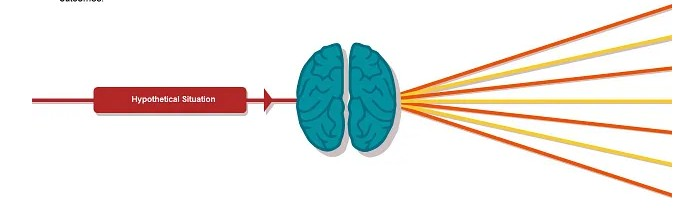
\includegraphics[width=0.5\linewidth,keepaspectratio]{mm7}
	\end{center}
	
{\tiny (Ref: The Art Of Thinking Clearly - Swabhav Tech Labs)}      
\end{frame}

%%%%%%%%%%%%%%%%%%%%%%%%%%%%%%%%%%%%%%%%%%%%%%%%%%%%%%%%%%%
\begin{frame}[fragile]\frametitle{Relativity}
  \begin{itemize}
    \item Perception depends on comparison.
    \item Not just physics , applies in psychology and economics.
    \item E.g., Rs.1000 seems big at a tea shop, small at Croma.
    \item Discounted MRPs manipulate perception of value.
    \item E.g., coaching institutes: ``Only Rs.1 lakh'' vs. ``Just 2 months' salary.''
    \item Avoid judging in isolation; watch your frame of reference.
  \end{itemize}
\end{frame}

%%%%%%%%%%%%%%%%%%%%%%%%%%%%%%%%%%%%%%%%%%%%%%%%%%%%%%%%%%%
\begin{frame}[fragile]\frametitle{Thermodynamics}
  \begin{itemize}
    \item Energy systems tend toward disorder (entropy).
    \item From physics; metaphor in organizational design.
    \item E.g., Indian government departments decay without active effort.
    \item Relationships degrade without energy (attention, care).
    \item E.g., neglected public infrastructure like Indian toilets, libraries.
    \item Systems must be fed with effort to counter entropy.
  \end{itemize}
\end{frame}

%%%%%%%%%%%%%%%%%%%%%%%%%%%%%%%%%%%%%%%%%%%%%%%%%%%%%%%%%%%
\begin{frame}[fragile]\frametitle{Inertia}
  \begin{itemize}
    \item Objects at rest stay at rest; systems resist change.
    \item From Newtonian physics; metaphor for habits, culture.
    \item Bureaucracies in India resist reform , status quo bias.
    \item People stick to routines despite better alternatives.
    \item E.g., cash use persists despite UPI in rural India.
    \item Momentum can be good or bad , be mindful of direction.
  \end{itemize}
\end{frame}

%%%%%%%%%%%%%%%%%%%%%%%%%%%%%%%%%%%%%%%%%%%%%%%%%%%%%%%%%%%
\begin{frame}[fragile]\frametitle{Friction and Viscosity}
  \begin{itemize}
    \item Resistance slows systems down.
    \item Physics origin, applied in design thinking.
    \item E.g., paperwork in Indian passport process adds friction.
    \item Online education failing due to tech/infrastructure drag.
    \item E.g., MSME loans delayed by regulatory viscosity.
    \item Reduce friction strategically, but preserve checks where needed.
  \end{itemize}
\end{frame}

%%%%%%%%%%%%%%%%%%%%%%%%%%%%%%%%%%%%%%%%%%%%%%%%%%%%%%%%%%%
\begin{frame}[fragile]\frametitle{Velocity}
  \begin{itemize}
    \item Speed in a particular direction.
    \item Physics model applied to business and policy.
    \item E.g., Indian startup growth = velocity, not just speed.
    \item Quick reforms + right direction = compounding effect.
    \item E.g., GST rollout aimed to increase fiscal velocity.
    \item Beware of high speed in wrong direction , causes more harm.
  \end{itemize}
\end{frame}

%%%%%%%%%%%%%%%%%%%%%%%%%%%%%%%%%%%%%%%%%%%%%%%%%%%%%%%%%%%
\begin{frame}[fragile]\frametitle{Leverage}
  \begin{itemize}
    \item Small inputs yielding large outputs.
    \item Originates from mechanics and finance.
    \item E.g., using tech (like UPI) to scale access to banking.
    \item Influencers use platforms to gain massive reach.
    \item Debt in real estate , high leverage in Indian housing boom.
    \item Use leverage carefully; too much can break the system.
  \end{itemize}
\end{frame}

%%%%%%%%%%%%%%%%%%%%%%%%%%%%%%%%%%%%%%%%%%%%%%%%%%%%%%%%%%%
\begin{frame}[fragile]\frametitle{Activation Energy}
  \begin{itemize}
    \item Minimum energy required to start a reaction.
    \item Chemistry origin; metaphor for habits and change.
    \item E.g., initial setup of solar in Indian homes is high, then payoff.
    \item Form-filling keeps citizens from accessing subsidies.
    \item E.g., waking up early needs energy ``spike'' at first.
    \item Lowering activation energy = increasing adoption.
  \end{itemize}
\end{frame}

%%%%%%%%%%%%%%%%%%%%%%%%%%%%%%%%%%%%%%%%%%%%%%%%%%%%%%%%%%%
\begin{frame}[fragile]\frametitle{Catalysts}
  \begin{itemize}
    \item Something that accelerates change without being consumed.
    \item From chemistry; used in transformation processes.
    \item E.g., a good mentor can catalyze career in Indian startups.
    \item Policies like Make in India as industrial catalysts.
    \item E.g., cricket coach who turns underdog into star.
    \item Catalysts don't guarantee success , they enable it.
  \end{itemize}
\end{frame}

%%%%%%%%%%%%%%%%%%%%%%%%%%%%%%%%%%%%%%%%%%%%%%%%%%%%%%%%%%%
\begin{frame}[fragile]\frametitle{Alloying}
  \begin{itemize}
    \item Combining elements for strength.
    \item From metallurgy; used metaphorically in teams/ideas.
    \item E.g., diverse coalition governments in India.
    \item Interdisciplinary education = alloy of skills.
    \item E.g., Hindi + tech = strong vernacular apps.
    \item Alloys may have trade-offs , balance strength vs. flexibility.
  \end{itemize}
\end{frame}

%%%%%%%%%%%%%%%%%%%%%%%%%%%%%%%%%%%%%%%%%%%%%%%%%%%%%%%%%%%
\begin{frame}[fragile]\frametitle{Evolution - Natural Selection}
  \begin{itemize}
    \item Survival of the fittest over generations.
    \item Darwinian principle; applicable to markets.
    \item Indian startups that adapt thrive (Zerodha, Paytm).
    \item Weak policies die out over time; strong ones stay.
    \item E.g., traditional farming surviving despite modern competition.
    \item Avoid romanticizing all survivors , some survive by chance.
  \end{itemize}
\end{frame}

%%%%%%%%%%%%%%%%%%%%%%%%%%%%%%%%%%%%%%%%%%%%%%%%%%%%%%%%%%%
\begin{frame}[fragile]\frametitle{Evolution - Adaptation}
  \begin{itemize}
    \item Organisms change to fit environment.
    \item Evolutionary biology principle.
    \item E.g., Indian retail moving from cash to QR codes.
    \item COVID forced remote working and online schooling.
    \item Small businesses adopted e-commerce or died.
    \item Adaptation is not always optimal , may be reactive.
  \end{itemize}
\end{frame}

%%%%%%%%%%%%%%%%%%%%%%%%%%%%%%%%%%%%%%%%%%%%%%%%%%%%%%%%%%%
\begin{frame}[fragile]\frametitle{Ecosystems}
  \begin{itemize}
    \item Interdependent networks of entities.
    \item From ecology; applied to business, tech.
    \item E.g., India's startup ecosystem: VCs, colleges, infra.
    \item Agriculture involves weather, soil, politics, supply chain.
    \item Bollywood = actors + OTT + media + fans.
    \item Don't isolate systems , analyze interactions.
  \end{itemize}
\end{frame}

%%%%%%%%%%%%%%%%%%%%%%%%%%%%%%%%%%%%%%%%%%%%%%%%%%%%%%%%%%%
\begin{frame}[fragile]\frametitle{Niches}
  \begin{itemize}
    \item Specialized roles within systems.
    \item From biology, used in marketing and strategy.
    \item E.g., Indian vernacular YouTubers targeting Tier-2 cities.
    \item Brands like Patanjali tapping Ayurvedic niche.
    \item Job roles like drone pilot, data annotator = new niches.
    \item Niches can be fragile , depend on broader system health.
  \end{itemize}
\end{frame}

%%%%%%%%%%%%%%%%%%%%%%%%%%%%%%%%%%%%%%%%%%%%%%%%%%%%%%%%%%%
\begin{frame}[fragile]\frametitle{Self-Preservation}
  \begin{itemize}
    \item Tendency of organisms/systems to protect themselves.
    \item Evolutionary instinct; metaphor in institutions.
    \item E.g., Indian babus resisting administrative reforms.
    \item People resist feedback that threatens ego.
    \item E.g., companies killing innovations to protect core business.
    \item Self-preservation is natural, but can block growth.
  \end{itemize}
\end{frame}

%%%%%%%%%%%%%%%%%%%%%%%%%%%%%%%%%%%%%%%%%%%%%%%%%%%%%%%%%%%
\begin{frame}[fragile]\frametitle{Replication}
  \begin{itemize}
    \item Ability to copy and scale reliably.
    \item From biology and manufacturing.
    \item E.g., Indian franchise model , CCD, Amul parlors.
    \item Education: coaching classes cloned in every city.
    \item E.g., political strategies replicated across states.
    \item Mindless replication can ignore local context.
  \end{itemize}
\end{frame}

%%%%%%%%%%%%%%%%%%%%%%%%%%%%%%%%%%%%%%%%%%%%%%%%%%%%%%%%%%%
\begin{frame}[fragile]\frametitle{Cooperation}
  \begin{itemize}
    \item Working together for mutual benefit.
    \item Core to human evolution and society.
    \item SHGs in India empowering rural women.
    \item Farmers pooling land/machinery.
    \item Swachh Bharat relied on mass cooperation.
    \item Needs trust, alignment , forced cooperation fails.
  \end{itemize}
\end{frame}

%%%%%%%%%%%%%%%%%%%%%%%%%%%%%%%%%%%%%%%%%%%%%%%%%%%%%%%%%%%
\begin{frame}[fragile]\frametitle{Hierarchical Organization}
  \begin{itemize}
    \item Systems structured in layers of control.
    \item Found in biology, military, governance.
    \item E.g., Indian bureaucracy: central, state, district levels.
    \item Companies with vertical vs. flat hierarchies.
    \item Indian family structures: elders → juniors.
    \item Hierarchy brings order, but can stifle speed and creativity.
  \end{itemize}
\end{frame}

%%%%%%%%%%%%%%%%%%%%%%%%%%%%%%%%%%%%%%%%%%%%%%%%%%%%%%%%%%%
\begin{frame}[fragile]\frametitle{Incentives}
  \begin{itemize}
    \item Behavior is shaped by rewards and penalties.
    \item Economics principle; vital in policy and business.
    \item E.g., LPG subsidy linked to Aadhaar = better targeting.
    \item Swiggy/Zomato drivers incentivized on deliveries.
    \item Voters swayed by freebie promises.
    \item Misaligned incentives = corruption, manipulation.
  \end{itemize}
\end{frame}

%%%%%%%%%%%%%%%%%%%%%%%%%%%%%%%%%%%%%%%%%%%%%%%%%%%%%%%%%%%
\begin{frame}[fragile]\frametitle{Tendency to Minimize Energy}
  \begin{itemize}
    \item Systems prefer the path of least resistance.
    \item Physics + human psychology.
    \item E.g., people choose WhatsApp forwards over research.
    \item Politicians use slogans instead of nuanced solutions.
    \item E.g., shortcuts in JEE prep , coaching hacks.
    \item Shortcuts are tempting , but costly if misused.
  \end{itemize}
\end{frame}

%%%%%%%%%%%%%%%%%%%%%%%%%%%%%%%%%%%%%%%%%%%%%%%%%%%%%%%%%%%
\begin{frame}[fragile]\frametitle{Feedback Loops}
  \begin{itemize}
    \item Outputs become new inputs, amplifying or correcting.
    \item From cybernetics; applies in economics, learning.
    \item E.g., social media likes → more posts → more likes.
    \item UPI usage loop: adoption → trust → more users.
    \item Crime in areas → police presence → less crime.
    \item Watch for both positive (amplifying) and negative (balancing) loops.
  \end{itemize}
\end{frame}

%%%%%%%%%%%%%%%%%%%%%%%%%%%%%%%%%%%%%%%%%%%%%%%%%%%%%%%%%%%%%%%%%%%%%%%%%%%%%%%%%%
\begin{frame}[fragile]\frametitle{}
\begin{center}
{\Large Building Your Personal Mental Models}

{\tiny (Ref: A Comprehensive Guide to Mental Models - Habits for Thinking)}

\end{center}
\end{frame}


%%%%%%%%%%%%%%%%%%%%%%%%%%%%%%%%%%%%%%%%%%%%%%%%%%%%%%%%%%%
\begin{frame}[fragile]\frametitle{Why Build a Latticework of Mental Models?}
  \begin{itemize}
	\item Latticework means interlocking structure of big ideas from different disciplines 
    \item Repeating mistakes? You're not alone.
    \item Best thinkers don't think harder,they think in models.
    \item A latticework = multiple models from various fields.
    \item Inspired by Charlie Munger's approach to decision-making.
    \item Models create clarity, prevent bias, and improve reasoning.
  \end{itemize}
\end{frame}

%%%%%%%%%%%%%%%%%%%%%%%%%%%%%%%%%%%%%%%%%%%%%%%%%%%%%%%%%%%
\begin{frame}[fragile]\frametitle{The Brain as a Workshop}
  \begin{itemize}
    \item Every mental model = a tool.
    \item Relying on one tool = repeated errors.
    \item Full toolkit = deeper insight + fewer blindspots.
    \item Munger: ``Array experience on a latticework of models.''
    \item Real decisions require multiple perspectives.
  \end{itemize}
\end{frame}

%%%%%%%%%%%%%%%%%%%%%%%%%%%%%%%%%%%%%%%%%%%%%%%%%%%%%%%%%%%
\begin{frame}[fragile]\frametitle{Why Interconnected Models Matter}
  \begin{itemize}
    \item Complex problems need multi-model solutions.
    \item Examples:
      \begin{itemize}
        \item Inversion (think backwards to prevent failure)
        \item 80/20 Rule (focus on leverage points)
        \item Second-order thinking (anticipate consequences)
      \end{itemize}
    \item Together: see around corners, think systemically.
  \end{itemize}
\end{frame}

%%%%%%%%%%%%%%%%%%%%%%%%%%%%%%%%%%%%%%%%%%%%%%%%%%%%%%%%%%%
\begin{frame}[fragile]\frametitle{Step 1: Cultivate Curiosity}
  \begin{itemize}
    \item Read across disciplines: psychology, biology, economics, etc.
    \item Look for timeless, transferable ideas.
    \item Ask: ``What's the principle here?''
    \item Apply ideas outside their original context.
    \item One book outside your comfort zone can shift your thinking.
  \end{itemize}
\end{frame}

%%%%%%%%%%%%%%%%%%%%%%%%%%%%%%%%%%%%%%%%%%%%%%%%%%%%%%%%%%%
\begin{frame}[fragile]\frametitle{Step 2: Actively Understand Models}
  \begin{itemize}
    \item Move from passive to active learning.
    \item Use the Feynman Technique: explain in plain language.
    \item Create analogies to what you know.
    \item Journal 3 uses per model.
    \item Seek cross-discipline examples for each model.
  \end{itemize}
\end{frame}

%%%%%%%%%%%%%%%%%%%%%%%%%%%%%%%%%%%%%%%%%%%%%%%%%%%%%%%%%%%
\begin{frame}[fragile]\frametitle{Step 3: Find Model Connections}
  \begin{itemize}
    \item Insight = when models intersect.
    \item Example intersections:
      \begin{itemize}
        \item Feedback loops + habit formation
        \item Marginal utility + diminishing returns
        \item Hanlon's Razor + Occam's Razor
      \end{itemize}
    \item Use mind maps or journals to visualize links.
    \item Practice with real decisions: apply 3 models at once.
  \end{itemize}
\end{frame}

%%%%%%%%%%%%%%%%%%%%%%%%%%%%%%%%%%%%%%%%%%%%%%%%%%%%%%%%%%%
\begin{frame}[fragile]\frametitle{Step 4: Practice \& Apply}
  \begin{itemize}
    \item Use models like lenses.
    \item Ask: ``What model fits this problem?''
    \item Try on everyday decisions:
      \begin{itemize}
        \item Weekly planning → Pareto Principle
        \item Disagreements → Steelman Technique
        \item Scheduling → Parkinson's Law
      \end{itemize}
    \item Repetition builds intuition.
  \end{itemize}
\end{frame}

%%%%%%%%%%%%%%%%%%%%%%%%%%%%%%%%%%%%%%%%%%%%%%%%%%%%%%%%%%%
\begin{frame}[fragile]\frametitle{Step 5: Review and Refine}
  \begin{itemize}
    \item Every quarter, reflect:
      \begin{itemize}
        \item Which models do I use most?
        \item Which still confuse me?
        \item What should I add next?
      \end{itemize}
    \item Keep a Mental Models Journal.
    \item Be willing to discard outdated models.
    \item Your latticework evolves with experience.
  \end{itemize}
\end{frame}

%%%%%%%%%%%%%%%%%%%%%%%%%%%%%%%%%%%%%%%%%%%%%%%%%%%%%%%%%%%
\begin{frame}[fragile]\frametitle{Overcoming Common Challenges}
  \begin{itemize}
    \item \textbf{Info Overload:} Start with 10 core models.
    \item \textbf{Time Constraints:} Use daily touchpoints,podcasts, short reads.
    \item \textbf{Shallow Learning:} Go deep, not wide.
    \item Value comes from mastery, not memory.
  \end{itemize}
\end{frame}

%%%%%%%%%%%%%%%%%%%%%%%%%%%%%%%%%%%%%%%%%%%%%%%%%%%%%%%%%%%
\begin{frame}[fragile]\frametitle{The Lifelong Edge}
  \begin{itemize}
    \item Your brain is a framework builder, not a sponge.
    \item A strong latticework lets you:
      \begin{itemize}
        \item Make better decisions
        \item Spot unseen patterns
        \item Avoid mental traps
        \item Communicate clearly
      \end{itemize}
    \item This is lifelong work. Build with care.
    \item Your mental toolkit is your edge.
  \end{itemize}
\end{frame}


%%%%%%%%%%%%%%%%%%%%%%%%%%%%%%%%%%%%%%%%%%%%%%%%%%%%%%%%%%%%%%%%%%%%%%%%%%%%%%%%%%
\begin{frame}[fragile]\frametitle{}
\begin{center}
{\Large Closure}
\end{center}
\end{frame}

%%%%%%%%%%%%%%%%%%%%%%%%%%%%%%%%%%%%%%%%%%%%%%%%%%%%%%%%%%%
\begin{frame}[fragile]\frametitle{Closure}
  \begin{itemize}
    \item A mental model is simply a representation of how something works. 
	\item We cannot keep all of the details of the world in our brains, so we use mental models to simplify the complex into understandable and organizable chunks.
  \end{itemize}
  
	\begin{center}
	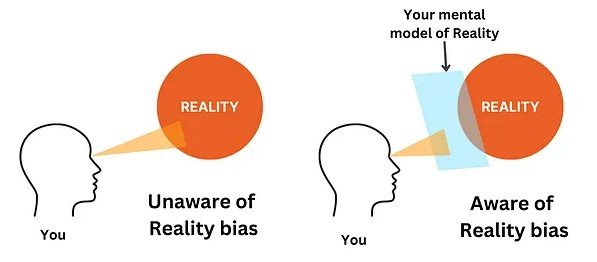
\includegraphics[width=0.8\linewidth,keepaspectratio]{mm2}
	\end{center}
	
{\tiny (Ref: The Art Of Thinking Clearly - Swabhav Tech Labs)}  
\end{frame}

%%%%%%%%%%%%%%%%%%%%%%%%%%%%%%%%%%%%%%%%%%%%%%%%%%%%%%%%%%%
\begin{frame}[fragile]\frametitle{References}
  \begin{itemize}
    \item Thinking, Fast and Slow by Daniel Kahneman
	\item Poor Charlie's Almanack edited by Peter D. Kaufman
	\item Super Thinking by Gabriel Weinberg \& Lauren McCann
	\item The Great Mental Models Series by Shane Parrish \& Rhiannon Beaubien (Farnam Street)
	\item Principles by Ray Dalio
  \end{itemize}

\end{frame}